\begin{abwframe}
\node[anchor=north west,inner sep=0pt,outer sep=0pt] at (506.126,-0) {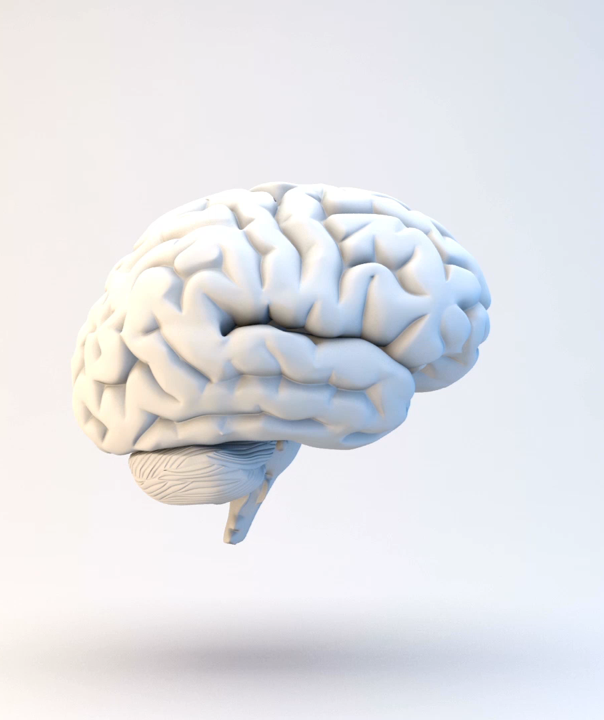
\includegraphics[width=452.914bp,height=540bp]{assets/source/slide-11-object-001.png}};
\node[anchor=north west,inner sep=0pt,outer sep=0pt] at (40.625,-55.791) {\begin{minipage}[t][69.584bp][c]{878.75bp}\setlength{\parindent}{0pt}\setlength{\parskip}{0pt}{\TimesNR\fontsize{44}{49.28}\selectfont\color{cBC0031}\bfseries\raggedright Neural networks\par}\end{minipage}};
\node[anchor=north west,inner sep=0pt,outer sep=0pt] at (56.693,-499.702) {\begin{minipage}[t][11.952bp][c]{324bp}\setlength{\parindent}{0pt}\setlength{\parskip}{0pt}{\TimesNR\fontsize{10}{11.2}\selectfont\color{c7F7F7F}\raggedright Analytics for a Better World Lecture 2\par}\end{minipage}};
\node[anchor=north west,inner sep=0pt,outer sep=0pt] at (880.898,-499.702) {\begin{minipage}[t][11.952bp][c]{22.409bp}\setlength{\parindent}{0pt}\setlength{\parskip}{0pt}{\TimesNR\fontsize{10}{11.2}\selectfont\color{c7F7F7F}\bfseries\raggedleft 11\par}\end{minipage}};
\node[anchor=north west,inner sep=0pt,outer sep=0pt] at (40.625,-158.857) {\begin{minipage}[t][299.652bp][c]{425.832bp}\setlength{\parindent}{0pt}\setlength{\parskip}{0pt}{\TimesNR\fontsize{24}{26.88}\selectfont\color{c000000}\raggedright This first part of the slide deck has been adapted from Lecture 12 from the course CSE 4309 – Machine Learning by Vassilis Athitsos at the Computer Science and Engineering Department of the University of Texas at Arlington\par}\end{minipage}};
\end{abwframe}
